\documentclass[twocolumn]{article}
\usepackage{amsmath}
\usepackage{amssymb}
\usepackage{amsthm}
\usepackage{amssymb}
\usepackage{mathdots}
\usepackage[pdftex]{graphicx}
\usepackage{fancyhdr}
\usepackage[margin=1in]{geometry}
\usepackage{multicol}
\usepackage{bm}
\usepackage{listings}
\PassOptionsToPackage{usenames,dvipsnames}{color}  %% Allow color names
\usepackage{pdfpages}
\usepackage{algpseudocode}
\usepackage{tikz}
\usepackage{enumitem}
\usepackage[T1]{fontenc}
\usepackage{inconsolata}
\usepackage{framed}
\usepackage{wasysym}
\usepackage[thinlines]{easytable}
\usepackage{wrapfig}
\usepackage{hyperref}
\usepackage{cancel}
\usepackage{tabu}
\usepackage{tcolorbox}
\usepackage{graphicx}
\usepackage{float}

\hypersetup{
    colorlinks=true,
    linkcolor=blue,
    filecolor=magenta,      
    urlcolor=cyan,
    pdfpagemode=FullScreen,
    }

\title{ARM Instruction Decoder and Lifter}
\author{Corey Wingo, Saffat Ahmed, Nolan Kuo, Jacob Wiedemeier}
\date{12/15/2022}

\rhead{}
\lfoot{}

\renewcommand{\headrulewidth}{0.4pt}
\renewcommand{\footrulewidth}{0.4pt}

\setlength{\parindent}{0pt}

\pagestyle{fancy}

\renewcommand{\thefootnote}{\fnsymbol{footnote}}

% start MZ
\usetikzlibrary{automata,positioning}
\let\oldemptyset\emptyset
\renewcommand{\emptyset}{\text{\O}}
\renewcommand\qedsymbol{$\blacksquare$}
\newenvironment{prf}{{\bfseries Proof.}}{\qedsymbol}
\renewcommand{\emph}[1]{\textit{\textbf{#1}}}
\newcommand{\annotate}[1]{\textit{\textcolor{blue}{#1}}}
\usepackage{stmaryrd}
% end MZ
\usepackage{pxfonts}

\lstset{language=Python,
    basicstyle=\ttfamily,
    keywordstyle=\bfseries,
    showstringspaces=false,
    morekeywords={include, printf}
}

\newenvironment{shadedbox}{\begin{tcolorbox}[width=\linewidth, sharp corners=all, colback=white!95!black]}{\end{tcolorbox}}
\usepackage{mathtools}
\DeclarePairedDelimiter\ceil{\lceil}{\rceil}
\DeclarePairedDelimiter\floor{\lfloor}{\rfloor}


\begin{document}

\maketitle


\section*{\centering Intro / Motivation}
\vspace{0.3cm}
The main focus of this project is the creation of a novel ARM instruction decoder and lifter that takes ARMv7 assembly and lifts it to an intermediary language (IL), Picanae in Coq in this case, that can be used for future works in proving the correctness of the ARM system.\\

ARM is the most widely used family of instruction set architectures, having a presence in the majority of smartphone processors. In addition, with Apple adopting the ARM architecture in its new M1 Chips, the need for security techniques that can guard against exploits is steadily increasing. Naturally, these techniques will need some way to verify correctness, hence the necessity of an ARM decoder and lifter.\\

To our knowledge, while there are Picanae systems that target similar architectures like RISCV, there is no ARM focused decoder that lifts instructions from a binary up to Picanae for usage in proofs of correctness. As such, our prototype system is novel in its targeted architecture and application. 

\section*{\centering Technical Approach}
\vspace{0.3cm}
We first approached the technical challenge of how to obtain the bytes to decode. Fortunately for us, as we are not supporting thumb mode, all ARMv7 instructions are 4 bytes long. However, as we are decoding ARMv7 binaries, we must be able to assemble ARMv7 instructions into their binary representation. For that, we used \href{https://cpulator.01xz.net/?sys=arm}{CPUlator} [1]. It can assemble ARMv7 instructions into their binary representations and even emulate them, as seen in Figure 1.\\

\begin{figure}[H]
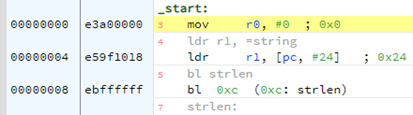
\includegraphics[width=\linewidth]{cpulator_example.png}\\
Figure 1. Assembly of ARMv7 instructions.
\centering
\end{figure}

We found that using the CPUlator tool was very tedious. It required us to manually copy and convert the hexadecimal bytes to decimal and then to paste it into the file. To mitigate this tedium, we tasked one of our members to write a tool that would grab the bytes directly from a binary and compile it into a COQ list that we could simply run.\\

We had to convert the representation of the assembled instructions from hexadecimal to decimal for compatability with the Picanae system. This did not change any of the operations we could perform on the representation. We can still use critical methods such as xbits and shift.\\

Once we have the instruction represented as a decimal, we are ready to decode it. In order to decode the instruction, we have to first understand the instruction encoding, as explained in the \href{https://developer.arm.com/documentation/ddi0406/c}{ARM Architecture Reference Manual} [2]. The architecture manual includes a chapter on how the instructions are precisely encoded down to the bit. It follows a tree-like structure of instruction types such as data-processing, load/store, branches, etc., as seen in Figure 2.  Once you’ve followed a branch by matching the specified bits, all instructions are of that type. This might go on for one or more recursive levels. This tree models a decision tree, where the internal nodes make decisions and the leaves are the instructions themselves, which are combinations of matches on the bits of its binary representation.\\
\begin{figure*}[!ht]
\centering
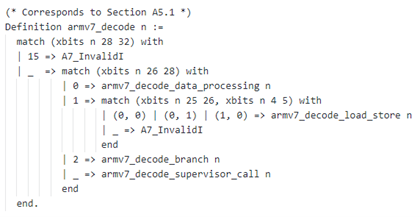
\includegraphics[width=.5\textwidth]{top-level_decode.png}\\
Figure 2. The top-level decoding definition.
\end{figure*}
After reading the reference manual for a few weeks, we had a general understanding of the characteristics of the encodings. A vast majority of the instructions encoding contained a 4-bit conditional value that represented the condition that the instruction should be executed on, such as EQUAL, NOT\_EQUAL, LESS\_THAN, ALWAYS, etc. These conditions are evaluated based on four flags: N, V, C, and Z. If the right flags are set then the condition is true and so the instruction is executed. However, almost all instructions other than the branches used the ALWAYS condition, so we opted to ignore the rest at the moment to focus our efforts at more critical points.\\

Another thing we learned was how common objects like registers and immediate values were encoded within the instruction bytes. Registers, which can range from r0, r1, …, r14 are represented as the 4-bit value 0, 1, …, 14, respectively. Immediate values are directly placed in the instruction bytes as 5, 12, or 16-bit values, usually on the lower-end side. Hence, grabbing the registers and immediate values was as simple as using xbits, as seen in Figure 3.\\

\begin{figure}[H]
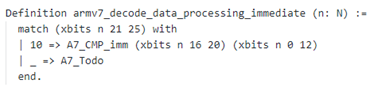
\includegraphics[width=\linewidth]{decode_immediate_example.png}\\
Figure 3. Example of decoding registers and immediates.
\centering
\end{figure}

Lifting the decoded instructions was straightforward when the instruction did not have any side effects, such as setting or getting flags. Without side effects, lifting an instruction was a simple mapping from the decoded instruction and its values (registers and immediates) to the lifted one.\\

Most instruction have side-effects, however. This includes setting certain flags within the ASPR register or setting certain registers to certain values in-addition to its primary effect. The solution to the former was verbose. Take the CMP instruction for example: if the value within the register minus the immediate value is zero, then set the Z flag to 1, otherwise set the Z flag to 0. There are 3 other flags that need to be set based on certain conditions as well, but for this example we will only look at the Z flag. We can model this in Picanae IL using If statements and expressions as seen in Figure 4 and Figure 5.\\

\begin{figure}[H]
\centering
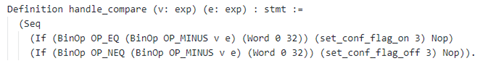
\includegraphics[width=\linewidth]{handle_compare_definition.png}\\
Figure 4. Part of the handle\_compare definition.


\end{figure}
\begin{figure}[H]
\centering
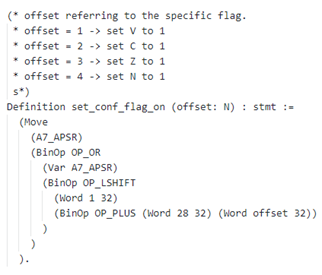
\includegraphics[width=.7\linewidth]{set_flag_example.png}\\
Figure 5. Setting a particular flag.

\end{figure}
With these side effects in mind, we were able to implement a structure that could generate a Picanae equivalent of the decoded ARMv7 instruction, with the IL statement generated fully describing the actions taken by the instruction on the processor, ie registers affected, operations executed, etc. The example provided in Figure 6 demonstrates how the decoded instructions correspond to their lifted counterpart. As you can see, the IL statement reveals all actions that the instruction is performing at time of execution, which is critical when proving correctness of a program's instructions.
\begin{figure*}[!ht]
\centering
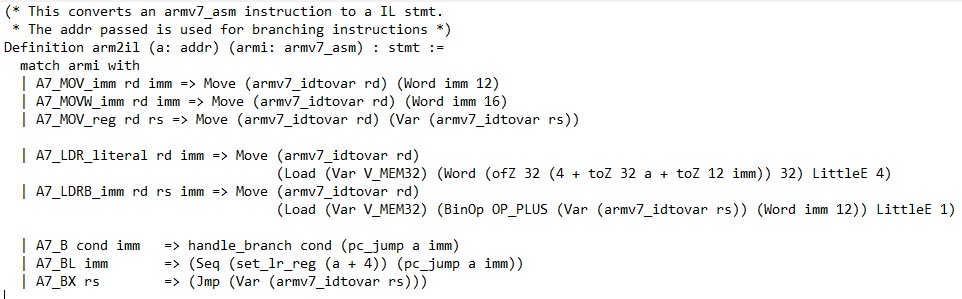
\includegraphics[width=0.8\linewidth]{arm2il_example.jpg}\\
Figure 6. Lifting decoded instructions to the intermediate language.

\end{figure*}

\newpage
\section*{\centering Team Organization}
\vspace{0.3cm}

\textbf{Corey Wingo}
\begin{itemize}
	\item Project leader
	\item Decoded and lifted a significant number of ARMv7 instructions
	\item Presenter\\
\end{itemize}


\textbf{Saffat Ahmed}
\begin{itemize}
	\item Decoded and lifted a significant number of ARMv7 instructions\\
\end{itemize}

\textbf{Nolan Kuo}
\begin{itemize}
	\item Decoded and lifted a significant number of ARMv7 instructions\\
\end{itemize}

\textbf{Jacob Wiedemeier}
\begin{itemize}
	\item Wrote a python script to generate a lookup table in Coq for individual opcodes in an ARMv7 binary
	\item Edited report and converted to LaTeX\\
\end{itemize}

\section*{\centering Evaluation}
\vspace{0.3cm}
Work and answer goes here

\section*{\centering Future Work}
\vspace{0.3cm}

The following list contains potential future work on the ARMv7 Decoder and Lifter. It is arranged in order of priority from top to bottom.\\
\begin{enumerate}
	\item Verify lifted instructions
	\item Add support for Thumb Mode
	\item Support all side effects of every instruction
	\item Support the entire instruction set\\
\end{enumerate}

Currently, we have not worked on verifying whether an instruction was lifted appropriately. A good method of verifying a lifted instruction would be running it within the Picanae System and observing its primary and side effects.\\

Supporting thumb mode is as simple as duplicating the existing code, except using encoding TX for the instruction within the ARMv7 Reference Manual. The decoding and lifting would need to be matched using different paths as they have different patterns and instruction parameters, such as different bit-width immediate values and registers. This would be tedious, but fairly easy, as you can reference the existing code.\\

We currently do not support every side effect for the instructions we lifted. For example, we ignore instruction variants that depend on conditional flags to execute. Another lack of implementation is the CMP instruction, which has an immense number of side-effects and represents an imposing challenge to decode and lift.\\

We do not support every instruction in the ARMv7 reference manual. There are about a hundred main instructions, each with many variants. We currently support approximately thirty main instructions.

\section*{\centering Related Work}
\vspace{0.3cm}

There are many ARMv7 decoders out there that we used as references on how to design such a decoder.\\

\href{https://github.com/iximeow/yaxpeax-arm}{Yaxpeax-arm} [3] is one such project that we referenced. Implemented in Rust, the project supports ARMv7, ARMv7/thumb, and aarch instruction sets. It can successfully decode and display the ARMv7 instruction from the actual instruction bytes through the usage of masking bytes and instruction logic. The source file also demonstrates the usage of a Thumb state for the decoder to keep track of the decoder state while processing instructions, which supports our expected future work regarding the support of thumb mode. Similar to our own implementation, their work does not have a formal method for proving the correctness of their instruction decoding. Instead, their verification involves exhaustive comparative tests on ARMv7 instructions with multiple proven decoders to verify the correctness of their decoder implementation - a process that will likely be mirrored in the future work of our own architecture.\\

We also very heavily relied on a previous implementation of a decoder and lifter for the Picanae system for the RISC-V architecture. The Picanae system provides a number of formally verified methods that allow projects to create decoder frameworks without needing to re-verify the correctness of methods, such as binary operations and bit extraction from a decimal number. The aforementioned RISC-V implementation was able to use these helper methods to extract instruction bytes in order to successfully decode and lift the RISC-V instruction set to the Picanae IL, providing a path to formal verification of RISC-V binaries. Since RISC-V has a simpler instruction set compared to ARMv7, we were able to utilize this implementation as the base template for our own implementation, with informal verification of our lifted instructions being compared to those from RISC-V to determine if the instruction behavior functioned similarly to our own.

\section*{\centering Citations}
\vspace{0.3cm}

[1] - CPUlator ARMv7 System Simulator. (2019, March 9). Retrieved December 13, 2022, from https://cpulator.01xz.net/?sys=arm\\

[2] - ARM Architecture Reference Manual ARMv7-A and ARMv7-R edition. arm Developer. (2011, November 23). Retrieved December 13, 2022, from https://developer.arm.com/documentation/ddi0406/c\\

[3] - Iximeow. (2022, September 29). Arm decoders for the Yaxpeax Project. GitHub. Retrieved December 13, 2022, from https://github.com/iximeow/yaxpeax-arm

\end{document}